
\documentclass[12pt,a4paper]{article}

%========================
% PAQUETES
%========================
\usepackage[utf8]{inputenc}
\usepackage[T1]{fontenc}
\usepackage[spanish,es-tabla]{babel}
\usepackage{amsmath, amssymb, amsfonts}
\usepackage{geometry}
\usepackage{booktabs}
\usepackage{array}
\usepackage{longtable}
\usepackage{multirow}
\usepackage{float}
\usepackage{graphicx}
\usepackage{setspace}
\usepackage{hyperref}
\usepackage{caption}
\usepackage{enumitem}
\usepackage{titlesec}
\usepackage{xcolor}
\usepackage{listings}
\usepackage{fancyhdr}

\geometry{left=2.8cm,right=2.5cm,top=2.5cm,bottom=2.5cm}
\onehalfspacing
\setlength{\parindent}{1.25cm}
\setlength{\parskip}{0.2cm}
% Evita desbordes de párrafo por palabras largas (p. ej. "tiempo×altura", rutas en \texttt)
\setlength{\emergencystretch}{3em}
\tolerance=1200
\hyphenpenalty=500

\graphicspath{{../codigo/figuras/}{figuras/}}

\hypersetup{
    colorlinks=true,
    linkcolor=blue,
    citecolor=blue,
    urlcolor=blue
}

\titleformat{\section}{\normalfont\Large\bfseries}{\thesection.}{0.5em}{}
\titleformat{\subsection}{\normalfont\large\bfseries}{\thesubsection.}{0.5em}{}
\titleformat{\subsubsection}{\normalfont\normalsize\bfseries}{\thesubsubsection.}{0.5em}{}

%========================
% ESTILO DE CÓDIGO PYTHON
%========================
\definecolor{codegray}{gray}{0.45}
\definecolor{codebg}{rgb}{0.97,0.97,0.97}
\definecolor{codekw}{rgb}{0.10,0.10,0.70}
\definecolor{codecom}{rgb}{0.20,0.50,0.25}
\definecolor{codestr}{rgb}{0.72,0.35,0.05}

\lstdefinestyle{python}{
    language=Python,
    backgroundcolor=\color{codebg},
    basicstyle=\ttfamily\footnotesize,
    keywordstyle=\color{codekw}\bfseries,
    commentstyle=\color{codecom}\itshape,
    stringstyle=\color{codestr},
    showstringspaces=false,
    breaklines=true,
    breakatwhitespace=false,
    breakindent=0pt,
    postbreak=\mbox{\textcolor{codegray}{$\hookrightarrow$}\space},
    frame=single,
    rulecolor=\color{codegray},
    numbers=left,
    numberstyle=\tiny\color{codegray},
    numbersep=8pt,
    % --- márgenes del bloque de código: marco y números dentro del área de texto ---
    xleftmargin=2.2em,
    framexleftmargin=2.2em,
    xrightmargin=0.8em,
    framexrightmargin=0pt,
    tabsize=4,
    captionpos=b,
    inputencoding=utf8,
    extendedchars=true,
    literate=%
      {á}{{\'a}}1 {é}{{\'e}}1 {í}{{\'i}}1 {ó}{{\'o}}1 {ú}{{\'u}}1
      {Á}{{\'A}}1 {É}{{\'E}}1 {Í}{{\'I}}1 {Ó}{{\'O}}1 {Ú}{{\'U}}1
      {ñ}{{\~n}}1 {Ñ}{{\~N}}1 {¿}{{?`}}1 {¡}{{!`}}1
      {×}{{$\times$}}1 {²}{{$^2$}}1 {°}{{$^\circ$}}1 {–}{{-}}1
}
\lstset{style=python}

%========================
% ENCABEZADO Y PIE DE PÁGINA
%========================
\setlength{\headheight}{15pt}
\pagestyle{fancy}
\fancyhf{}
\fancyhead[L]{\small\itshape Examen --- Diseño factorial}
\fancyhead[R]{\small\itshape Efectos fijos, aleatorios y mixtos}
\fancyfoot[C]{\thepage}
\fancyfoot[R]{\scriptsize\ttfamily resolucion\_factorial}
\renewcommand{\headrulewidth}{0.4pt}
\renewcommand{\footrulewidth}{0.2pt}

%========================
% DATOS DEL INFORME
%========================
\title{
\textbf{Resolución del examen mediante diseños factoriales}\\
\large Análisis del arreglo factorial $2\times3\times3$ bajo efectos fijos, aleatorios y mixtos, y comparación con el DCA, para la inactivación de \textit{Escherichia coli} y \textit{Salmonella typhimurium} mediante radiación UV-C
}

\author{
Curso: Métodos Estadísticos para Investigaciones Experimentales\\
Escuela de Posgrado -- Unidad de Posgrado en Ciencias Físicas y Matemáticas\\
Universidad Nacional de Trujillo
}

\date{\today}

\begin{document}

%========================
% CARÁTULA
%========================
\begin{titlepage}
\centering
\thispagestyle{empty}

{\scshape\Large Universidad Nacional de Trujillo\par}
\vspace{0.35cm}
{\scshape\large Escuela de Posgrado\par}
{\scshape Unidad de Posgrado en Ciencias Físicas y Matemáticas\par}
\vspace{0.6cm}
\rule{\textwidth}{1.0pt}

\vfill

{\Huge\bfseries Resolución del examen\\mediante diseños factoriales\par}
\vspace{1.0cm}
{\large\itshape Análisis del arreglo factorial $2\times3\times3$ bajo
\textbf{efectos fijos, aleatorios y mixtos}, y su comparación con el diseño
completamente al azar, para la inactivación de
\textmd{\textit{Escherichia coli}} y \textmd{\textit{Salmonella typhimurium}}
mediante radiación UV-C en carne de cuy\par}

\vspace{1.0cm}
\rule{0.55\textwidth}{0.6pt}

\vfill

{\large
\setlength{\tabcolsep}{2pt}
\begin{tabular}{r@{\hspace{0.8em}}l}
\textbf{Curso:}      & Métodos Estadísticos para Investigaciones Experimentales\\[6pt]
\textbf{Docente:}    & Dr. Roger Reyna Segura\\[6pt]
\textbf{Estudiante:} & Rudy Franklin Condori Quilla\\[6pt]
\textbf{Programa:}   & Posgrado en Ciencias Físicas y Matemáticas\\
\end{tabular}\par}

\vfill

{\small Condiciones del modelo analizadas: efectos fijos, efectos aleatorios y efectos mixtos.\par}
\vspace{0.5cm}
\rule{\textwidth}{1.0pt}
\vspace{0.3cm}
{\large Trujillo -- Perú\par}
{\large \the\year{}\par}

\end{titlepage}

%========================
% NOTA DE LECTURA
%========================
\begin{quote}
\small \textbf{Cómo leer este informe.} Esta es la \emph{segunda} resolución del examen, centrada en el \textbf{diseño factorial}. Parte del mismo experimento del primer informe, pero desarrolla el arreglo factorial $2\times3\times3$ bajo las \textbf{tres condiciones} del archivo \texttt{condiciones.txt}: \textbf{efectos fijos}, \textbf{efectos aleatorios} y \textbf{efectos mixtos}. Cada modelo se presenta en tres capas: \textbf{(a)~resolución manual} (modelo, hipótesis y reglas de los cuadrados medios esperados), \textbf{(b)~script de Python} que reproduce el análisis, y \textbf{(c)~resultados y explicación}. Además, cada sección sigue la secuencia: \textbf{Paso 1} preparar o resumir, \textbf{Paso 2} ejecutar y \textbf{Paso 3} interpretar. Todos los valores provienen del notebook reproducible \texttt{codigo/analisis\_factorial.ipynb} y son \emph{coherentes con los datos del primer examen}.
\end{quote}

\newpage
\tableofcontents
\newpage

%========================
\section{Introducción}

El primer examen auditó la tesis \textit{«Radiación UV-C para inactivar patógenos alimentarios \textit{Escherichia coli} y \textit{Salmonella typhimurium} en carne de cuy contaminado»}, concluyó que el diseño declarado (preexperimental) era inadecuado y propuso un \textbf{diseño completamente al azar (DCA) con arreglo factorial $2\times3\times3$} como modelo recomendado. La mejor opción \emph{operativa} del primer examen, dentro de esa familia, fue el DCA que trata las nueve combinaciones tiempo$\times$altura como nueve tratamientos.

Esta segunda resolución profundiza en el \textbf{arreglo factorial}. El objetivo es desarrollar el factorial $2\times3\times3$ bajo las \textbf{tres condiciones} del modelo lineal indicadas en \texttt{condiciones.txt} ---\textbf{efectos fijos}, \textbf{efectos aleatorios} y \textbf{efectos mixtos}---, determinar cuál es el mejor modelo factorial y compararlo con la mejor opción de DCA obtenida en el primer examen.

La idea central es que las tres condiciones \textbf{comparten la misma descomposición de sumas de cuadrados}, pero difieren en los \textbf{cuadrados medios esperados (EMS)}, que determinan cuál es el \textbf{denominador correcto} de cada prueba $F$. Como se verá, esta elección cambia las conclusiones sobre los efectos principales, mientras que la interacción tiempo$\times$altura permanece como el efecto robusto del experimento.

\subsection{Síntesis de los modelos del primer examen}

Como antecedente, la Tabla~\ref{tab:resumen-examen1} resume los \textbf{seis modelos} evaluados en el primer examen, con su modelo estadístico, su resultado principal y su veredicto. Esta segunda resolución retoma de allí el \textbf{arreglo factorial} (modelos 5 y 6) y lo profundiza bajo las tres condiciones del modelo lineal; al final (Sección~\ref{sec:factorial-vs-dca}) se compara el mejor modelo factorial con la mejor opción de DCA (modelo 2).

\begin{longtable}{>{\raggedright\arraybackslash}p{1.9cm}>{\raggedright\arraybackslash}p{3.4cm}>{\raggedright\arraybackslash}p{4.5cm}>{\raggedright\arraybackslash}p{2.9cm}}
\caption{Resumen de los modelos evaluados en el primer examen.}\label{tab:resumen-examen1}\\
\toprule
\textbf{Modelo} & \textbf{Modelo estadístico} & \textbf{Resultado principal} & \textbf{Veredicto}\\
\midrule
\endfirsthead
\multicolumn{4}{l}{\small\itshape (continuación de la Tabla \ref{tab:resumen-examen1})}\\
\toprule
\textbf{Modelo} & \textbf{Modelo estadístico} & \textbf{Resultado principal} & \textbf{Veredicto}\\
\midrule
\endhead
\midrule
\multicolumn{4}{r}{\small\itshape continúa en la página siguiente}\\
\endfoot
\bottomrule
\endlastfoot
1. Preexperimental & $Y_{ij}=\mu+\tau_i+e_{ij}$ (control vs.\ tratado) & UV-C reduce la carga $\approx95\%$ ($t$ de Welch, $p\ll0{,}001$) & Insuficiente: no evalúa tiempo, altura ni interacción\\
\addlinespace
2. DCA & $Y_{ij}=\mu+\tau_i+e_{ij}$ (9 tratamientos) & Tratamientos significativos ($F=23{,}45$ y $26{,}42$; $p<0{,}001$) & Válido, pero no separa los efectos\\
\addlinespace
3. DBCA & $Y_{ij}=\mu+\tau_i+\beta_j+e_{ij}$ (bloque = réplica) & Bloques \textbf{no} significativos ($p=0{,}59$ y $0{,}76$) & No mejora al DCA; bloqueo injustificado\\
\addlinespace
4. Cuadrado latino & $Y_{ijk}=\mu+\tau_i+\rho_j+\gamma_k+e_{ijk}$ & Confundiría la interacción ($141{,}3$) con el error & \textbf{Inaplicable}: tiempo y altura son factores, no bloques\\
\addlinespace
5. Factorial $3\times3$ (por microorg.) & $Y_{ijk}=\mu+\alpha_i+\beta_j+(\alpha\beta)_{ij}+e_{ijk}$ & Tiempo, altura e interacción significativos ($R^2\approx0{,}88$) & Muy adecuado por microorganismo\\
\addlinespace
6. Factorial $2\times3\times3$ & Modelo~\eqref{eq:modelo} (completo) & Significativos $A$, $B$, $C$, $A\times B$ y, dominante, $B\times C$ ($F=52{,}76$) & \textbf{Recomendado} (el más completo)\\
\end{longtable}

%========================
\section{Objetivos}

\subsection{Objetivo general}

Resolver el experimento de radiación UV-C mediante el arreglo factorial $2\times3\times3$, analizándolo bajo las condiciones de efectos fijos, aleatorios y mixtos, y comparar el mejor modelo factorial con la mejor opción de DCA del primer examen.

\subsection{Objetivos específicos}

\begin{enumerate}[label=\alph*)]
    \item Plantear el modelo factorial y la descomposición de sumas de cuadrados común a las tres condiciones.
    \item Formular, para cada condición, los cuadrados medios esperados y las pruebas $F$ correctas.
    \item Resolver el factorial bajo efectos fijos (Modelo I).
    \item Resolver el factorial bajo efectos aleatorios (Modelo II), incluyendo la estimación de componentes de varianza.
    \item Resolver el factorial bajo efectos mixtos (Modelo III).
    \item Seleccionar el mejor modelo factorial con criterios estadísticos y de pertinencia científica.
    \item Comparar el mejor modelo factorial con la mejor opción de DCA del primer examen.
    \item Validar los supuestos y formular las conclusiones.
\end{enumerate}

%========================
\section{Estructura factorial y datos}

Se conserva el conjunto de datos del primer examen: 72 observaciones tratadas (los controles $T(0)$--$H(0)$ se usaron en el primer informe para el modelo preexperimental). El arreglo factorial cruza tres factores:

\begin{table}[H]
\centering
\caption{Factores del arreglo factorial.}
\begin{tabular}{llc}
\toprule
\textbf{Factor} & \textbf{Niveles} & \textbf{Símbolo}\\
\midrule
Microorganismo & \textit{E. coli}, \textit{S. typhimurium} & $A$ ($a=2$)\\
Tiempo de exposición & 1, 3, 5 min & $B$ ($b=3$)\\
Altura o distancia & 5, 10, 20 cm & $C$ ($c=3$)\\
Repeticiones por celda & M1--M4 & $n=4$\\
\bottomrule
\end{tabular}
\end{table}

La variable respuesta es el recuento de sobrevivientes en placa (UFC). El total es $N=a\,b\,c\,n=2\times3\times3\times4=72$. Los datos ordenados están en \texttt{codigo/datos\_uvc.csv}.

%========================
\section{Marco teórico: efectos fijos, aleatorios y mixtos}

El modelo del arreglo factorial de tres factores con interacción es
\begin{equation}
Y_{ijkl} = \mu + A_i + B_j + C_k + (AB)_{ij} + (AC)_{ik} + (BC)_{jk} + (ABC)_{ijk} + \varepsilon_{ijkl},
\label{eq:modelo}
\end{equation}
con $i=1,\dots,a$; $j=1,\dots,b$; $k=1,\dots,c$; $l=1,\dots,n$ y $\varepsilon_{ijkl}\sim N(0,\sigma^2)$.

La \textbf{descomposición de la suma de cuadrados} es la misma en las tres condiciones:
\[
SC_{tot}=SC_A+SC_B+SC_C+SC_{AB}+SC_{AC}+SC_{BC}+SC_{ABC}+SC_E .
\]
Lo que cambia es la \textbf{naturaleza de los términos} y, con ella, los \textbf{cuadrados medios esperados (EMS)}, que fijan el denominador de cada $F$.

\subsection{Modelo I --- efectos fijos}

Los niveles de cada factor son los \emph{únicos} de interés. Los efectos son constantes sujetas a $\sum A_i=\sum B_j=\cdots=0$. Todo efecto se contrasta contra el error:
\[
E(CM_{efecto})=\sigma^2+\text{(forma cuadrática del efecto)}
\quad\Rightarrow\quad
F=\frac{CM_{efecto}}{CM_{E}} .
\]

\subsection{Modelo II --- efectos aleatorios}

Los niveles son una muestra aleatoria de una población de niveles; cada efecto es una variable aleatoria con su componente de varianza ($\sigma^2_A,\sigma^2_B,\dots$). Las hipótesis se plantean sobre las varianzas ($H_0:\sigma^2_{efecto}=0$). Los EMS hacen que:
\[
F_{ABC}=\frac{CM_{ABC}}{CM_E},\qquad
F_{AB}=\frac{CM_{AB}}{CM_{ABC}},\quad
F_{AC}=\frac{CM_{AC}}{CM_{ABC}},\quad
F_{BC}=\frac{CM_{BC}}{CM_{ABC}},
\]
y los efectos principales \textbf{no tienen prueba $F$ exacta}: requieren un denominador sintético de \textbf{Satterthwaite}, p.\,ej.
\[
F_A=\frac{CM_A}{CM_{AB}+CM_{AC}-CM_{ABC}},\qquad
\nu=\frac{(CM_{AB}+CM_{AC}-CM_{ABC})^2}{\dfrac{CM_{AB}^2}{gl_{AB}}+\dfrac{CM_{AC}^2}{gl_{AC}}+\dfrac{CM_{ABC}^2}{gl_{ABC}}} .
\]
Los \textbf{componentes de varianza} se estiman por el método de los momentos igualando $CM$ a $EMS$:
\[
\begin{aligned}
\hat\sigma^2&=CM_E, & \qquad
\hat\sigma^2_{ABC}&=\frac{CM_{ABC}-CM_E}{n},\\[4pt]
\hat\sigma^2_{BC}&=\frac{CM_{BC}-CM_{ABC}}{a\,n}, & \qquad
\hat\sigma^2_{A}&=\frac{CM_{A}-CM_{AB}-CM_{AC}+CM_{ABC}}{b\,c\,n},
\end{aligned}
\]
y análogamente para los demás términos.

\subsection{Modelo III --- efectos mixtos}

Algunos factores son fijos y otros aleatorios. Se adopta el escenario más razonable para este experimento: \textbf{microorganismo ($A$) fijo} ---los dos patógenos de interés sanitario--- y \textbf{tiempo ($B$) y altura ($C$) aleatorios} ---una muestra de los ajustes operativos posibles de la cámara UV-C. Bajo el \emph{modelo restringido}, las reglas de EMS conducen a:
\[
F_A=\frac{CM_A}{CM_{AB}+CM_{AC}-CM_{ABC}},\qquad
F_B=\frac{CM_B}{CM_{BC}},\qquad
F_C=\frac{CM_C}{CM_{BC}},
\]
\[
F_{AB}=\frac{CM_{AB}}{CM_{ABC}},\quad
F_{AC}=\frac{CM_{AC}}{CM_{ABC}},\qquad
F_{BC}=\frac{CM_{BC}}{CM_E},\quad
F_{ABC}=\frac{CM_{ABC}}{CM_E}.
\]

%========================
\section{ANOVA factorial base (descomposición común)}

\subsection{Resolución manual}

Con $a=2$, $b=3$, $c=3$, $n=4$, los grados de libertad son: $A=1$, $B=2$, $C=2$, $AB=2$, $AC=2$, $BC=4$, $ABC=4$ y error $=abc(n-1)=18\cdot3=54$. Esta tabla de cuadrados medios es el \textbf{insumo común} de los tres modelos.

\subsection{Script en Python}

\begin{lstlisting}[caption={Descomposición factorial y extracción de cuadrados medios.}]
modelo = ols("recuento ~ C(microorganismo)*C(tiempo)*C(altura)", data=df).fit()
tab = anova_lm(modelo, typ=2)            # diseño balanceado: typ 1 = 2 = 3
SC = {k: tab.loc[v,"sum_sq"] for k,v in key.items()}
GL = {k: int(tab.loc[v,"df"]) for k,v in key.items()}
MS = {k: SC[k]/GL[k] for k in SC}
\end{lstlisting}

\subsection{Resultados}

\begin{table}[H]
\centering
\caption{Descomposición de sumas de cuadrados del factorial $2\times3\times3$ ($R^2=0{,}885$; $R^2_{adj}=0{,}848$).}
\begin{tabular}{lrrr}
\toprule
\textbf{Fuente} & \textbf{SC} & \textbf{gl} & \textbf{CM}\\
\midrule
$A$: microorganismo            & 19.014  & 1  & 19.014\\
$B$: tiempo                    & 172.194 & 2  & 86.097\\
$C$: altura                    & 117.361 & 2  & 58.681\\
$A\times B$                    & 44.528  & 2  & 22.264\\
$A\times C$                    & 1.694   & 2  & 0.847\\
$B\times C$ (tiempo$\times$altura) & 378.139 & 4  & 94.535\\
$A\times B\times C$            & 9.639   & 4  & 2.410\\
Error                          & 96.750  & 54 & 1.792\\
\bottomrule
\end{tabular}
\end{table}

\subsection{Explicación}

La suma de cuadrados más grande con diferencia es la de la \textbf{interacción tiempo$\times$altura} ($SC_{BC}=378{,}1$), seguida del tiempo y la altura. Estos cuadrados medios alimentan las tres condiciones; solo cambia el denominador de cada $F$.

%========================
\section{Modelo I --- Efectos fijos}

\subsection{Resolución manual}

Los dos microorganismos, los tres tiempos y las tres alturas son los \emph{únicos} de interés. Hipótesis (forma genérica): $H_0$: todos los efectos del término son nulos; $H_1$: al menos uno no lo es. Cada $F$ usa $CM_E=1{,}792$ (gl $=54$) como denominador.

\subsection{Script en Python}

\begin{lstlisting}[caption={Pruebas F del modelo de efectos fijos (todo contra el error).}]
for k in ["A","B","C","AB","AC","BC","ABC"]:
    F = MS[k]/MS["E"];  p = stats.f.sf(F, GL[k], GL["E"])
\end{lstlisting}

\subsection{Resultados}

\begin{table}[H]
\centering
\caption{ANOVA factorial $2\times3\times3$ --- \textbf{efectos fijos} (denominador: $CM_E$).}
\begin{tabular}{lrccc}
\toprule
\textbf{Fuente} & \textbf{$F$} & \textbf{gl} & \textbf{p-valor} & \textbf{Signif.}\\
\midrule
$A$: microorganismo            & 10.612 & (1, 54) & 0.0019 & *\\
$B$: tiempo                    & 48.054 & (2, 54) & $<0.001$ & *\\
$C$: altura                    & 32.752 & (2, 54) & $<0.001$ & *\\
$A\times B$                    & 12.426 & (2, 54) & $<0.001$ & *\\
$A\times C$                    & 0.473  & (2, 54) & 0.626  & ns\\
$B\times C$ (tiempo$\times$altura) & 52.764 & (4, 54) & $<0.001$ & *\\
$A\times B\times C$            & 1.345  & (4, 54) & 0.265  & ns\\
\bottomrule
\end{tabular}
\end{table}

\subsection{Explicación}

Son significativos microorganismo, tiempo, altura, la interacción microorganismo$\times$tiempo y, de forma \textbf{dominante}, la interacción \textbf{tiempo$\times$altura} ($F=52{,}76$). No son significativas microorganismo$\times$altura ni la interacción triple. Este resultado coincide con el modelo factorial recomendado del primer examen.

%========================
\section{Modelo II --- Efectos aleatorios}

\subsection{Resolución manual}

Si los niveles fueran una muestra aleatoria, las pruebas seguirían las reglas de EMS de la Sección~4.2: las interacciones dobles se contrastan contra la triple, la triple contra el error, y los efectos principales contra denominadores sintéticos de Satterthwaite. Por ejemplo, para $A$:
\[
F_A=\frac{CM_A}{CM_{AB}+CM_{AC}-CM_{ABC}}=\frac{19{,}01}{22{,}26+0{,}85-2{,}41}=\frac{19{,}01}{20{,}70}=0{,}92 .
\]

\subsection{Script en Python}

\begin{lstlisting}[caption={Pruebas F del modelo aleatorio y componentes de varianza.}]
def f_satterthwaite(num, mas, menos):
    den = sum(MS[t] for t in mas) - sum(MS[t] for t in menos)
    gl_den = den**2 / sum((MS[t]**2)/GL[t] for t in (mas+menos))
    return MS[num]/den, GL[num], gl_den, stats.f.sf(MS[num]/den, GL[num], gl_den)

sigma2_BC = (MS["BC"] - MS["ABC"]) / (a*n)      # componente de varianza de la interaccion
\end{lstlisting}

\subsection{Resultados}

\begin{table}[H]
\centering
\caption{ANOVA factorial --- \textbf{efectos aleatorios} (denominadores según EMS).}
\begin{tabular}{lrccl}
\toprule
\textbf{Fuente} & \textbf{$F$} & \textbf{gl} & \textbf{p-valor} & \textbf{Denominador}\\
\midrule
$A$: microorganismo & 0.918 & (1, 1.72) & 0.453 & $CM_{AB}+CM_{AC}-CM_{ABC}$\\
$B$: tiempo         & 0.753 & (2, 5.27) & 0.516 & $CM_{AB}+CM_{BC}-CM_{ABC}$\\
$C$: altura         & 0.631 & (2, 3.87) & 0.579 & $CM_{AC}+CM_{BC}-CM_{ABC}$\\
$A\times B$         & 9.239 & (2, 4)    & 0.032 & $CM_{ABC}$\\
$A\times C$         & 0.352 & (2, 4)    & 0.723 & $CM_{ABC}$\\
$B\times C$         & 39.231& (4, 4)    & 0.0018& $CM_{ABC}$\\
$A\times B\times C$ & 1.345 & (4, 54)   & 0.265 & $CM_{E}$\\
\bottomrule
\end{tabular}
\end{table}

\begin{table}[H]
\centering
\caption{Componentes de varianza (método de los momentos). Un valor negativo se interpreta como cero.}
\begin{tabular}{lrr}
\toprule
\textbf{Componente} & \textbf{Estimación} & \textbf{\% del total no negativo}\\
\midrule
$\sigma^2_{BC}$ (tiempo$\times$altura) & 11.516  & 76.2\,\%\\
$\sigma^2$ (error)                     & 1.792   & 11.9\,\%\\
$\sigma^2_{AB}$                        & 1.654   & 10.9\,\%\\
$\sigma^2_{ABC}$                       & 0.155   & 1.0\,\%\\
$\sigma^2_{AC}$                        & $-0.130$ & 0\,\%\\
$\sigma^2_{A}$ (microorganismo)        & $-0.047$ & 0\,\%\\
$\sigma^2_{B}$ (tiempo)                & $-1.179$ & 0\,\%\\
$\sigma^2_{C}$ (altura)                & $-1.429$ & 0\,\%\\
\bottomrule
\end{tabular}
\end{table}

\subsection{Explicación}

Bajo el modelo aleatorio cambian las conclusiones: los \textbf{efectos principales dejan de ser significativos} (se contrastan contra denominadores grandes con muy pocos grados de libertad), mientras que la \textbf{interacción tiempo$\times$altura} sigue siendo significativa. Aparecen \textbf{componentes de varianza negativos} (microorganismo, tiempo, altura), señal inequívoca de que el supuesto de ``niveles aleatorios'' \textbf{no es coherente} con estos datos; además, el $76\%$ de la varianza no negativa se concentra en la interacción tiempo$\times$altura.

%========================
\section{Modelo III --- Efectos mixtos}

\subsection{Resolución manual}

Microorganismo $A$ fijo; tiempo $B$ y altura $C$ aleatorios (modelo restringido, Sección~4.3). El efecto fijo $A$ usa el denominador sintético; $B$ y $C$ se contrastan contra $CM_{BC}$; las interacciones con $A$ contra $CM_{ABC}$; y $BC$ y $ABC$ contra el error. Por ejemplo:
\[
F_B=\frac{CM_B}{CM_{BC}}=\frac{86{,}10}{94{,}53}=0{,}91,\qquad
F_{BC}=\frac{CM_{BC}}{CM_E}=\frac{94{,}53}{1{,}79}=52{,}76 .
\]

\subsection{Script en Python}

\begin{lstlisting}[caption={Pruebas F del modelo mixto restringido (A fijo; B, C aleatorios).}]
F_A,_,gA,pA = f_satterthwaite("A", ["AB","AC"], ["ABC"])  # efecto fijo
F_B = MS["B"]/MS["BC"];   F_C = MS["C"]/MS["BC"]           # aleatorios vs CM_BC
F_BC = MS["BC"]/MS["E"];  F_ABC = MS["ABC"]/MS["E"]        # vs error
\end{lstlisting}

\subsection{Resultados}

\begin{table}[H]
\centering
\caption{ANOVA factorial --- \textbf{efectos mixtos} ($A$ fijo; $B$, $C$ aleatorios; restringido).}
\begin{tabular}{lrccl}
\toprule
\textbf{Fuente} & \textbf{$F$} & \textbf{gl} & \textbf{p-valor} & \textbf{Denominador}\\
\midrule
$A$: microorganismo & 0.918  & (1, 1.72) & 0.453 & $CM_{AB}+CM_{AC}-CM_{ABC}$\\
$B$: tiempo         & 0.911  & (2, 4)    & 0.472 & $CM_{BC}$\\
$C$: altura         & 0.621  & (2, 4)    & 0.582 & $CM_{BC}$\\
$A\times B$         & 9.239  & (2, 4)    & 0.032 & $CM_{ABC}$\\
$A\times C$         & 0.352  & (2, 4)    & 0.723 & $CM_{ABC}$\\
$B\times C$         & 52.764 & (4, 54)   & $<0.001$ & $CM_{E}$\\
$A\times B\times C$ & 1.345  & (4, 54)   & 0.265 & $CM_{E}$\\
\bottomrule
\end{tabular}
\end{table}

\subsection{Explicación}

En el modelo mixto, la \textbf{interacción tiempo$\times$altura vuelve a ser muy significativa} ($F=52{,}76$, contra el error), pero los efectos principales tiempo y altura \textbf{no} lo son al contrastarse contra $CM_{BC}$. La interacción microorganismo$\times$tiempo se mantiene significativa. Aun cambiando el supuesto sobre los factores, \textbf{la interacción tiempo$\times$altura es el efecto robusto} del experimento.

%========================
\section{Comparación de las tres condiciones}

\begin{table}[H]
\centering
\caption{Valor $F$ (y decisión) de cada efecto bajo las tres condiciones. * $=p<0{,}05$; ns $=$ no significativo.}
\begin{tabular}{lccc}
\toprule
\textbf{Efecto} & \textbf{Fijos (I)} & \textbf{Aleatorios (II)} & \textbf{Mixtos (III)}\\
\midrule
$A$: microorganismo & 10.61 (*) & 0.92 (ns) & 0.92 (ns)\\
$B$: tiempo         & 48.05 (*) & 0.75 (ns) & 0.91 (ns)\\
$C$: altura         & 32.75 (*) & 0.63 (ns) & 0.62 (ns)\\
$A\times B$         & 12.43 (*) & 9.24 (*)  & 9.24 (*)\\
$A\times C$         & 0.47 (ns) & 0.35 (ns) & 0.35 (ns)\\
$B\times C$         & 52.76 (*) & 39.23 (*) & 52.76 (*)\\
$A\times B\times C$ & 1.35 (ns) & 1.35 (ns) & 1.35 (ns)\\
\bottomrule
\end{tabular}
\end{table}

\begin{figure}[H]
\centering
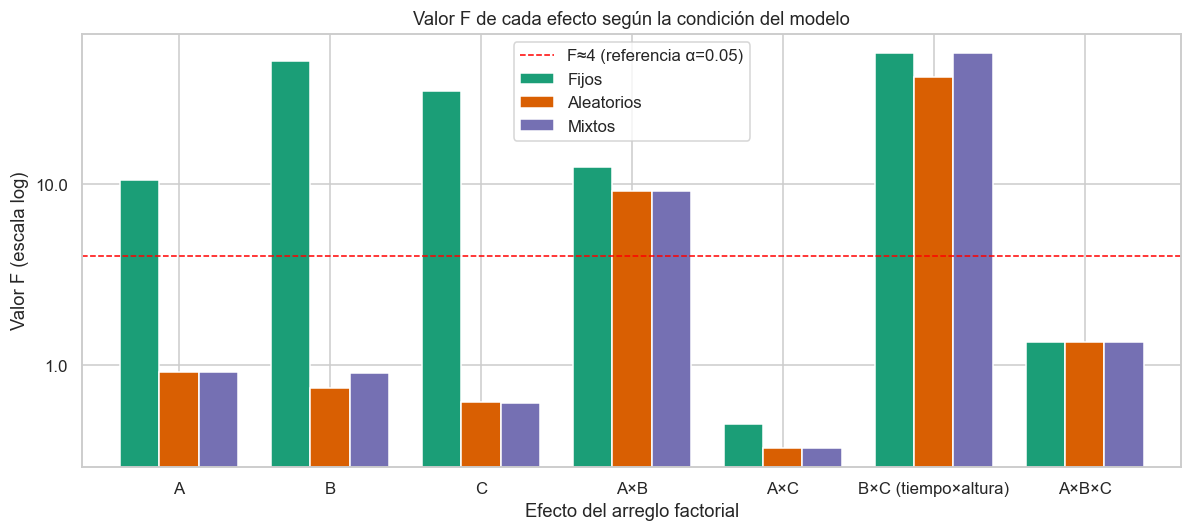
\includegraphics[width=0.95\textwidth]{03_F_por_condicion.png}
\caption{Valor $F$ de cada efecto según la condición del modelo (escala logarítmica). La interacción tiempo$\times$altura ($B\times C$) supera la referencia en los tres modelos: es el efecto robusto. Los efectos principales caen por debajo del umbral al tratarse como aleatorios o mixtos.}
\end{figure}

La interacción \textbf{tiempo$\times$altura} es significativa en las tres condiciones. Los efectos principales, en cambio, solo son significativos bajo efectos fijos: al pasar a aleatorios o mixtos se contrastan contra la propia interacción y pierden potencia. \textbf{La conclusión depende del supuesto fijos/aleatorios/mixtos.}

%========================
\section{Componentes de varianza e interacción}

\begin{figure}[H]
\centering
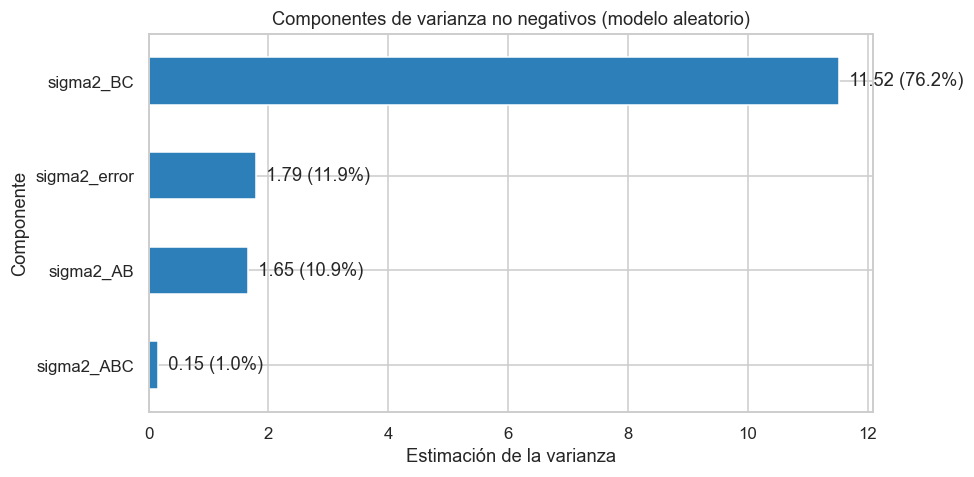
\includegraphics[width=0.9\textwidth]{04_componentes_varianza.png}
\caption{Componentes de varianza no negativos (modelo aleatorio). La interacción tiempo$\times$altura concentra el $76\%$ de la varianza.}
\end{figure}

\begin{figure}[H]
\centering
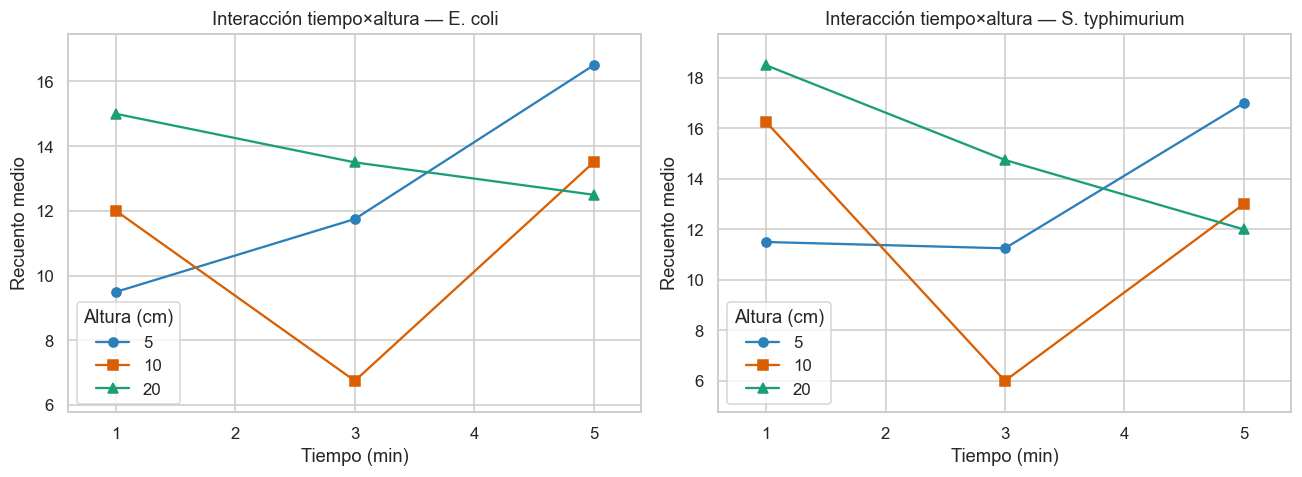
\includegraphics[width=0.95\textwidth]{05_interaccion_tiempo_altura.png}
\caption{Gráficos de interacción tiempo$\times$altura por microorganismo. Las líneas se cruzan: a 10 cm el recuento cae fuertemente a los 3 min (óptimo), mientras que 5 cm y 20 cm se comportan distinto.}
\end{figure}

%========================
\section{Selección del mejor modelo factorial}

\begin{longtable}{>{\raggedright\arraybackslash}p{2.5cm}>{\raggedright\arraybackslash}p{3.7cm}>{\raggedright\arraybackslash}p{3.5cm}>{\raggedright\arraybackslash}p{2.3cm}}
\caption{Comparación de las tres condiciones del modelo factorial.}\\
\toprule
\textbf{Modelo} & \textbf{Comportamiento estadístico} & \textbf{Pertinencia científica} & \textbf{Veredicto}\\
\midrule
\endfirsthead
\toprule
\textbf{Modelo} & \textbf{Comportamiento estadístico} & \textbf{Pertinencia científica} & \textbf{Veredicto}\\
\midrule
\endhead
Efectos fijos (I) & Todos los efectos vs.\ error (gl $=54$): máxima potencia & Coherente: los niveles fueron fijados por el investigador & \textbf{$\bigstar$ Recomendado}\\
Efectos aleatorios (II) & Denominadores con 4 gl y Satterthwaite ($\sim2$ gl): poca potencia; componentes de varianza \textbf{negativos} & Solo válido si los niveles fueran una muestra aleatoria & No adecuado\\
Efectos mixtos (III) & Efectos principales vs.\ $CM_{BC}$: poca potencia & Defendible solo si se generaliza a rangos continuos de tiempo y altura & Parcial / discutible\\
\bottomrule
\end{longtable}

\textbf{Decisión.} El \textbf{mejor modelo factorial es el de efectos fijos (Modelo I)}. Los niveles de los tres factores fueron \textbf{seleccionados deliberadamente} (dos patógenos de interés sanitario y valores concretos de tiempo y altura), por lo que la inferencia se dirige a \emph{esos} niveles y no a una población. Además, los modelos aleatorio y mixto producen \textbf{componentes de varianza negativos} y denominadores con muy pocos grados de libertad (potencia baja e inestable), lo que confirma que el supuesto de aleatoriedad no es apropiado para este experimento.

%========================
\section{Comparación: mejor factorial (fijos) vs.\ mejor DCA del primer examen}
\label{sec:factorial-vs-dca}

\subsection{Resolución manual}

La mejor opción del primer examen fue el \textbf{DCA} que trata las nueve combinaciones tiempo$\times$altura como nueve tratamientos (ANOVA de una vía por microorganismo). El factorial \textbf{descompone} esa suma de cuadrados de tratamientos:
\[
SC_{trat}^{DCA}=SC_{tiempo}+SC_{altura}+SC_{tiempo\times altura}.
\]
Para \textit{E. coli}: $74{,}00+52{,}17+141{,}33=267{,}50=SC_{trat}$. Para \textit{S. typhimurium}: $142{,}72+66{,}89+246{,}44=456{,}06=SC_{trat}$. El error y el $R^2$ son idénticos.

\subsection{Script en Python}

\begin{lstlisting}[caption={DCA (una vía) frente al factorial 3x3, por microorganismo.}]
m_dca = ols("recuento ~ C(trat)", data=sub).fit()              # 9 tratamientos
m_fac = ols("recuento ~ C(tiempo)*C(altura)", data=sub).fit()  # descomposicion
# misma SSE y mismo R2; el factorial separa tiempo, altura e interaccion
\end{lstlisting}

\subsection{Resultados}

\begin{table}[H]
\centering
\caption{DCA frente a factorial $3\times3$ por microorganismo (misma SSE y mismo $R^2$).}
\begin{tabular}{llrrrrr}
\toprule
\textbf{Microorg.} & \textbf{Fuente} & \textbf{Tiempo} & \textbf{Altura} & \textbf{T$\times$A} & \textbf{SSE} & \textbf{$R^2$}\\
\midrule
\textit{E. coli} & $SC_{trat}^{DCA}=267{,}50$ & 74.00 & 52.17 & 141.33 & 38.50 & 0.874\\
\textit{S. typhimurium} & $SC_{trat}^{DCA}=456{,}06$ & 142.72 & 66.89 & 246.44 & 58.25 & 0.887\\
\bottomrule
\end{tabular}
\end{table}

\begin{figure}[H]
\centering
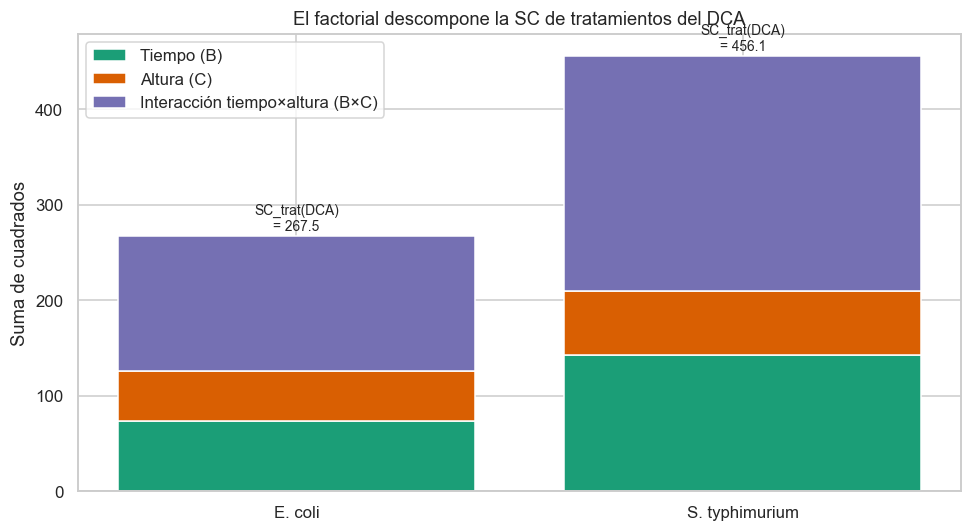
\includegraphics[width=0.85\textwidth]{06_factorial_vs_dca.png}
\caption{El factorial descompone la suma de cuadrados de tratamientos del DCA en tiempo, altura e interacción tiempo$\times$altura, conservando el mismo error.}
\end{figure}

\begin{table}[H]
\centering
\caption{Comparación final: mejor DCA vs.\ mejor modelo factorial.}
\begin{tabular}{p{3.2cm}p{4.2cm}p{4.6cm}}
\toprule
\textbf{Modelo} & \textbf{Resultado principal} & \textbf{Veredicto}\\
\midrule
DCA (1 vía, 9 tratamientos) & Detecta diferencias entre tratamientos ($p<0{,}001$) & Válido, pero agregado: no separa los factores\\
Factorial fijos $2\times3\times3$ & Cuantifica $A$, $B$, $C$ y todas las interacciones; misma SSE y $R^2$ & \textbf{Superior: identifica la interacción tiempo$\times$altura}\\
\bottomrule
\end{tabular}
\end{table}

\subsection{Explicación}

El factorial de efectos fijos \textbf{no compite} con el DCA: lo \textbf{contiene}. Con el mismo costo experimental y el mismo error, el factorial entrega \textbf{más información}, pues revela que el efecto del tiempo depende de la altura (interacción dominante). El \textbf{factorial de efectos fijos es el mejor modelo}.

%========================
\section{Validación de supuestos del modelo seleccionado}

Sobre los residuos del modelo factorial de efectos fijos:

\begin{lstlisting}[caption={Normalidad (Shapiro--Wilk) y homocedasticidad (Levene).}]
W, p = stats.shapiro(modelo.resid)
grupos = [g.recuento.values for _, g in df.groupby(["microorganismo","trat"])]
L, p = stats.levene(*grupos, center="median")
\end{lstlisting}

\begin{table}[H]
\centering
\caption{Pruebas de supuestos sobre el modelo factorial de efectos fijos.}
\begin{tabular}{>{\raggedright\arraybackslash}p{3.7cm}>{\raggedright\arraybackslash}p{2.5cm}>{\raggedright\arraybackslash}p{4.2cm}>{\raggedright\arraybackslash}p{2.4cm}}
\toprule
\textbf{Supuesto} & \textbf{Prueba} & \textbf{Estadístico / p-valor} & \textbf{Decisión}\\
\midrule
Normalidad de residuos & Shapiro--Wilk & $W=0{,}969$;\ $p=0{,}069$ & No se rechaza\\
Homogeneidad de varianzas & Levene (18 grupos) & $\text{stat}=0{,}547$;\ $p=0{,}915$ & Se cumple\\
\bottomrule
\end{tabular}
\end{table}

\begin{figure}[H]
\centering
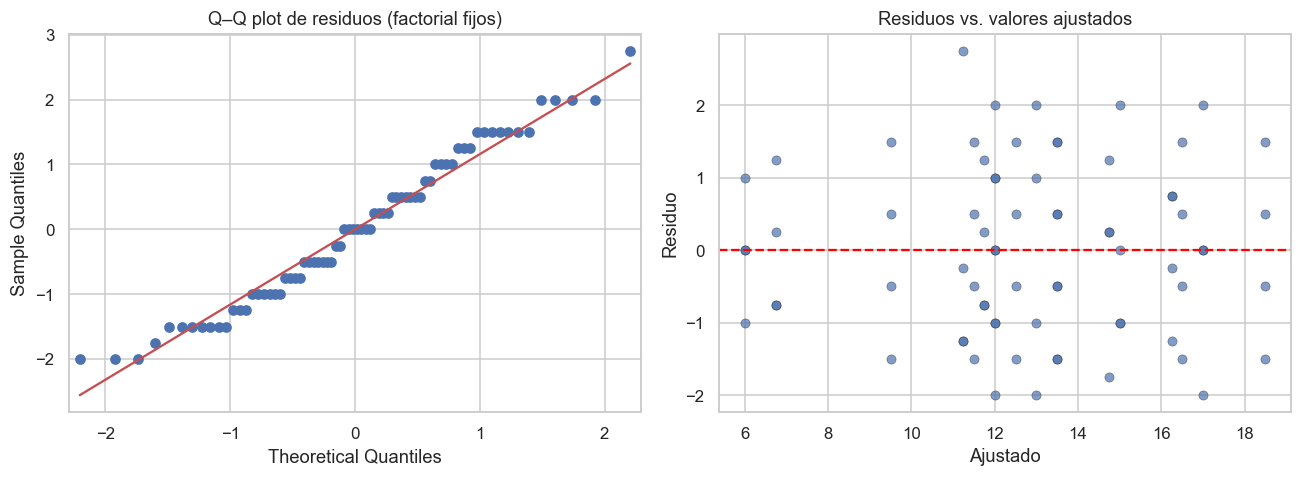
\includegraphics[width=0.95\textwidth]{07_diagnostico_residuos.png}
\caption{Q--Q plot (los puntos siguen la recta) y residuos vs.\ ajustados (nube sin patrón ni embudo): los supuestos se satisfacen razonablemente.}
\end{figure}

%========================
\section{Comparaciones múltiples (Tukey HSD)}

Como la interacción tiempo$\times$altura es significativa, el tratamiento óptimo se identifica por combinación de niveles. Se aplica Tukey sobre los nueve tratamientos por microorganismo.

\begin{table}[H]
\centering
\caption{Resumen de Tukey HSD (etiquetas T\textit{tiempo}\_H\textit{altura}).}
\begin{tabular}{lcc}
\toprule
\textbf{Microorganismo} & \textbf{Mejor (menor recuento)} & \textbf{Peor}\\
\midrule
\textit{E. coli} & T3\_H10 (3 min--10 cm): 6.75 & T5\_H5: 16.50\\
\textit{S. typhimurium} & T3\_H10 (3 min--10 cm): 6.00 & T1\_H20: 18.50\\
\bottomrule
\end{tabular}
\end{table}

Tukey confirma que \textbf{3 min -- 10 cm} produce el menor recuento en ambos patógenos, en coherencia con el primer examen.

%========================
\section{Conclusiones}

\begin{enumerate}
    \item El arreglo factorial $2\times3\times3$ admite tres lecturas (fijos, aleatorios y mixtos) que \textbf{comparten las sumas de cuadrados} pero difieren en los \textbf{denominadores} de las pruebas $F$.
    \item \textbf{Efectos fijos:} son significativos microorganismo, tiempo, altura, $A\times B$ y, de forma dominante, la \textbf{interacción tiempo$\times$altura} ($F=52{,}76$).
    \item \textbf{Efectos aleatorios:} los efectos principales pierden significancia y surgen \textbf{componentes de varianza negativos}; el supuesto no es coherente con los datos.
    \item \textbf{Efectos mixtos:} la \textbf{interacción tiempo$\times$altura sigue muy significativa}; los efectos principales no lo son frente a $CM_{BC}$.
    \item \textbf{Efecto robusto:} la interacción tiempo$\times$altura es significativa en las tres condiciones.
    \item \textbf{Mejor modelo factorial: efectos fijos}, por la naturaleza deliberada de los niveles y por la inestabilidad de los modelos aleatorio/mixto.
    \item \textbf{Factorial vs.\ DCA:} el factorial de efectos fijos \textbf{contiene} al DCA del primer examen (misma SSE y $R^2$) y además descompone la variación en tiempo, altura e interacción $\Rightarrow$ es \textbf{superior}.
    \item \textbf{Supuestos:} normalidad global aceptable ($p=0{,}069$) y homogeneidad de varianzas holgada ($p=0{,}915$).
    \item \textbf{Tratamiento óptimo:} \textbf{3 min -- 10 cm} en ambos patógenos (recuentos $6{,}75$ y $6{,}00$), confirmado por Tukey.
\end{enumerate}

%========================
\section{Respuesta final}

Resuelto el experimento como arreglo factorial $2\times3\times3$ bajo las tres condiciones del modelo, se concluye que el \textbf{mejor modelo factorial es el de efectos fijos}, porque los niveles de microorganismo, tiempo y altura fueron elegidos deliberadamente y la inferencia se dirige a esos niveles; los modelos de efectos aleatorios y mixtos resultan inadecuados (componentes de varianza negativos y denominadores con muy pocos grados de libertad). La \textbf{interacción tiempo$\times$altura} es el efecto robusto, significativo en las tres condiciones. Comparado con la mejor opción del primer examen, el factorial de efectos fijos \textbf{contiene al DCA} ---misma suma de cuadrados del error y mismo $R^2$--- pero lo \textbf{supera} al descomponer la variación en sus fuentes e identificar la interacción. El tratamiento óptimo es \textbf{3 minutos a 10 cm} para ambos patógenos.

%========================
\section*{Reproducibilidad}
\addcontentsline{toc}{section}{Reproducibilidad}

Todos los resultados, tablas y figuras se generan ejecutando el notebook \texttt{codigo/analisis\_factorial.ipynb}:

\begin{lstlisting}[language=bash,caption={Reconstrucción del análisis factorial.}]
cd resolucion_factorial/codigo
pip install -r requirements.txt
python build_notebook.py                                    # (re)genera el notebook
jupyter nbconvert --to notebook --execute --inplace analisis_factorial.ipynb
\end{lstlisting}

%========================
\section*{Referencias básicas sugeridas}
\addcontentsline{toc}{section}{Referencias básicas sugeridas}

\begin{itemize}
    \item Montgomery, D. C. (2019). \textit{Design and Analysis of Experiments}. Wiley. (Cap.\ de modelos aleatorios y mixtos en factoriales.)
    \item Kuehl, R. O. (2001). \textit{Diseño de experimentos: principios estadísticos para el diseño y análisis de investigaciones}. Thomson.
    \item Steel, R. G. D., Torrie, J. H., \& Dickey, D. A. (1997). \textit{Principles and Procedures of Statistics: A Biometrical Approach}. McGraw-Hill.
    \item Gutiérrez Pulido, H. y De la Vara Salazar, R. (2012). \textit{Análisis y diseño de experimentos}. McGraw-Hill.
\end{itemize}

\end{document}
